% !TEX encoding = UTF-8
% !TEX TS-program = pdflatex
% !TEX root = ../main.tex
% !TEX spellcheck = en-GB

\documentclass[final, 11pt, a4paper, titlepage]{article}
\makeatletter
\AtBeginDocument{\let\hl\@firstofone}
\makeatother

\usepackage[english]{babel}
\usepackage[utf8]{inputenc}
\usepackage[hidelinks]{hyperref}
\usepackage{graphicx}
\usepackage{textcomp}
\usepackage{wallpaper}
\usepackage{color}
\usepackage{mathtools}
\usepackage{listings}
\usepackage{amssymb}
\usepackage[
	backend=biber,
	citestyle=numeric-comp,
	hyperref,
	backref,
	sorting=none
]{biblatex}

\graphicspath{{images/}}

\addbibresource{bibliography.bib}


\defbibheading{bibliography}
{
    \phantomsection 
    \addcontentsline{toc}{section}{\bibname}
    \section*{\bibname\markboth{\bibname}{\bibname}}
}

\setlength\bibitemsep{1.5\itemsep} 

%\DeclareBibliographyCategory{sampleCategory}

%\addtocategory{sampleCategory}{referenceID}


\newcommand{\university}{Università degli Studi di Padova}
\newcommand{\dept}{Department of Mathematics}
\newcommand{\faculty}{Master Degree in Computer Science}
\newcommand{\myyear}{Academic Year 2016/17}
\renewcommand{\title}{QuizFight}
\newcommand{\subtitle}{An Android trivia quiz application}
\newcommand{\fstauthor}{Alex Beccaro - 1156235}
\newcommand{\sndauthor}{Emanuele Carraro - 1155105}
\newcommand{\trdauthor}{Matteo Di Pirro - 1154231}

\begin{document}
	\begin{titlepage}
\begin{center}

\begin{LARGE}
\textbf{\university}\\
\end{LARGE}

\vspace{10pt}

\begin{Large}
\textsc{\dept}\\
\end{Large}

\vspace{10pt}

\begin{large}
\textsc{\faculty}\\
\end{large}

\vspace{30pt}
\begin{figure}[htbp]
\begin{center}

\includegraphics[height=6cm]{images/logo_unipd}
\end{center}
\end{figure}
\vspace{30pt} 

\begin{LARGE}
\begin{center}
\textbf{\title}\\
\end{center}
\end{LARGE}

\begin{Large}
	\begin{center}
		\textbf{\subtitle}\\
	\end{center}
\end{Large}

\vspace{20pt} 

\begin{large}
\begin{flushright}
\textit{\fstauthor \\ \sndauthor \\ \trdauthor}
\end{flushright}
\end{large}

\vspace{40pt}

\line(1, 0){338} \\
\begin{normalsize}
\textsc{\myyear}
\end{normalsize}

\end{center}
\end{titlepage} 
	\tableofcontents
	\newpage
	\section{QuizFight server}

QuizFight relies on a Node.js server and a MongoDB database.
We choose these technologies consequently to the choice of the JSON format for
exchanging data.
In fact, since Node.js uses JavaScript as a language, it is well suited for
dealing with JSON messages.
The same motivation applies for MongoDB. It is a NoSQL database, where
documents can be thought as JSON files.
The flexibility of both communication and saving convinced us to use this
stack.
Furthermore there are no strong evidences, based on performance and overhead,
against the use of a Node.js server rather that a Java one. 

To interact with the database we use a well-known Node.js's package:
\texttt{mongoose.js}.
By following the Model-View-Controller design pattern we define both
models and controllers server side and let the clients provide the View-part.

For exposing our APIs, we use \texttt{Express.js}.
Each API is represented by a \texttt{Route} object.
No access is directly made from the routes to the model objects.
Instead, they use some methods provided by the controllers, exactly as stated
by the MVC pattern.

The server is a fundamental component in QuizFight. In fact, it is used to
store the data of the users and duels, and it also performs the binding
$<$player, opponent$>$ and keeps the actual questions.
Duels are thus generated server side and sent, on demand, to the clients,
round by round.

Users identification is based on their GGames usernames.
This provides an effective way to retrieve their information and to bind
them in duels.
We could have used MongoDB identifiers, instead we used usernames for their
simplicity.
In fact, using MongoDB's ids would have required too much effort.
Clients are unaware of how the server identifies users, so in this case the
best we could do client side is to send usernames.
Then, on the server, for each operation involving users we should have
retrieved user's information.
This pattern, although possible, rapidly deteriorates to a lot of unnecessary
requests.
We then prefer using usernames, which we know by Google's assurance to be
unique.

\subsection{Client-server communication}
For communicating with the server we chose the Retrofit library. It is a 
type-safe REST client for Android (or just Java) developed by Square. 
It provides a powerful framework for interacting with APIs and sending 
network requests with the HTTP client \texttt{OkHttp}. Its request/response
API is designed with fluent builders and immutability. It supports both 
synchronous blocking calls and async calls with callbacks. 

This library makes downloading JSON or XML data from a web API fairly 
straightforward. Once the data is downloaded then it is parsed into a 
Plain Old Java Object (POJO) which must be defined for each ``resource'' 
in the response.

The communication obviously requires the \texttt{android.permission.INTERNET}
permission. We share only JSON objects. As aforementioned, our server is 
specifically designed for being efficient in JSON handling. Even if a 
communication paradigm based on XML would be more secure (as XML has a schema
defining exactly how the document should be), the JSON alternative is simpler 
and faster. Furthermore, we do not need an absolute confidence in the document. If
one or more required fields are missing, the server notifies the client using an
error response.

Using JSON arises a problem at client side. Java is a strongly typed language, so we
cannot freely manipulate objects as in JavaScript. We need a way to cast a JSON 
object into a Java (POJO) one. We do that using Gson, a Google's library for 
serializing and deserializing JSON objects. 

Following the object-oriented programming paradigm we design a scalable and easily 
manageable architecture for REST calls. Figure~\ref{fig:retrofit} shows a partial
class diagram for that. Only two concrete API calls are shown; for the others it 
is exactly the same.
\begin{figure}[h]
	\centering
	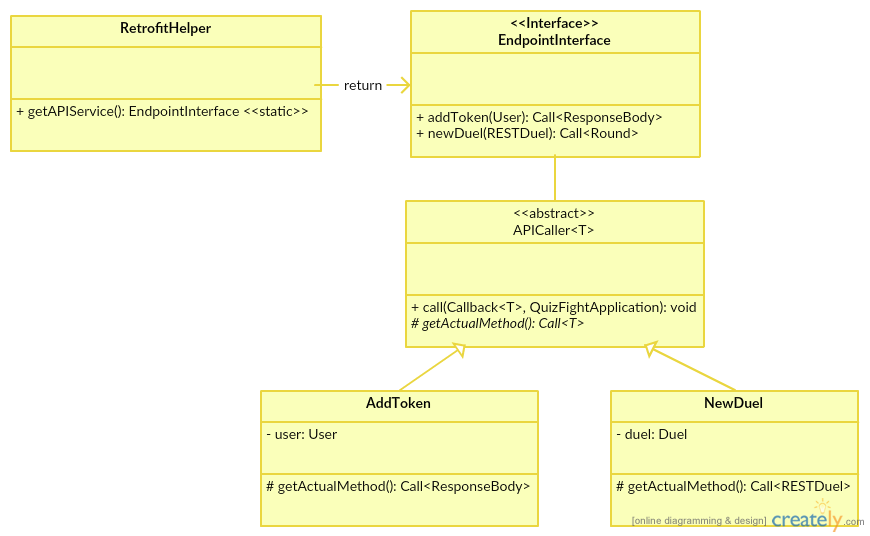
\includegraphics[width=0.9\linewidth]{Retrofit}
	\caption{High-level class diagram for API calls}
	\label{fig:retrofit}
\end{figure}

\texttt{RetrofitHelper} is the actual entry point. Its method \texttt{getAPIService()}
configures every parameter required, such as the base URL, the timeout, and the 
library for dealing with JSON. Then, via reflection, it creates on the fly a 
concrete \texttt{EndpointInterface} instance. The latter actually contains the
methods corresponding to the API calls. Retrofit allows us to specify HTTP
parameters by using Java-based annotations, such as \texttt{@Headers} for the
headers, and \texttt{@PUT("endpoint")} for a PUT call. 

Those methods return a generic \texttt{Call<T>} object. The type parameter 
represents the POJO object returned by the server. In this sense Retrofit is a
type-safe REST library. The \texttt{EndpointInterface} concrete instance is then
used by an abstract class, \texttt{APICaller}, which basically implements a mix
of the template method and command design patterns. Each concrete class extending
\texttt{APICall} should have a field representing the object to be sent, 
as a parameter, to the server. Then it implements the abstract method 
\texttt{getActualMethod()} in order to make the right call with the right 
parameters. It is invoked by the \texttt{APICall}'s \texttt{call()} method,
which also enqueues the actual execution to be performed in an asynchronous way. 

Then, whenever a Java class wishes to communicate with the server, it must 
instantiate the corresponding API class, give a parameter to it and provide
two callbacks, \texttt{onResponse()} and \texttt{onFailure()}, for handling the
corresponding situations. Listing~\ref{lst:servercall} shows an example.

\begin{lstlisting}[language=Java, caption={Server call example}, label={lst:servercall}]
new AddToken(new User(
	Games.Players.getCurrentPlayer(client).getDisplayName(),
	token,
	Secure.getString(getContentResolver(), Secure.ANDROID_ID)
)).call(new Callback<ResponseBody>() {
	@Override
	public void onResponse(Call<ResponseBody> call, Response<ResponseBody> response) {}
	
	@Override
	public void onFailure(Call<ResponseBody> call, Throwable t) {}
}, getApplication());
\end{lstlisting}	
	
	%%bibliography
	%\newpage
	%\nocite{*}
	%\printbibliography 
	
\end{document}